%
% Chapter Introduction
%
\chapter{User Guide}
The next chapters will guide you through the funktions of Dicomux. You will find
out the concept of dicomux and the way to use it.

\section{Workspace}
	The main concept od DICOMUX is the workspace. Every file or directory has its
	own workspace. When you open a dicom file or a dicom directory DICOMUX opens for
	you a new workspace. The workspace is shown as independend tab. Changes in a
	workspace have no effect to other workspaces. The welcome workspace is the
	default workspace. DICOMUX shows at least one workspace. If no other workspace
	is open, DICOMUX shows the default workspace.\\
	
	\begin{minipage}{\textwidth}
	\centering
	\fbox{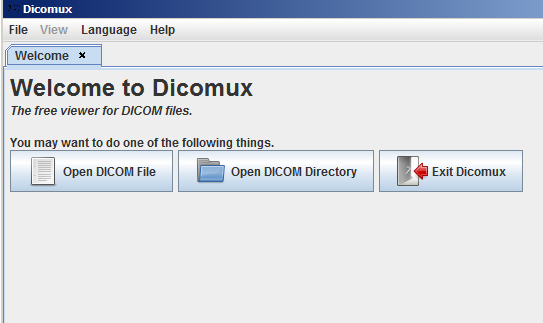
\includegraphics{screens/workspaceWelcome.png}}
	\captionof{figure}{Default workspace}
	\end{minipage}

	
	\subsection{Views}
	Every workspace of a file has different views. A view shows
	different parts of a dicom file.
	Some views supported by DICOMUX are Raw Data, Encapsulated PDF, Waveform ECG,
	etc.. For example shows the Encapsulated PDF view the encapsualted pdf file of
	the dicom file. If the dicom file doesn` t have a encapsulated pdf, the view
	Encapsulated PDF is not available.\\
	
	\begin{minipage}{\textwidth} 
	\centering
	\fbox{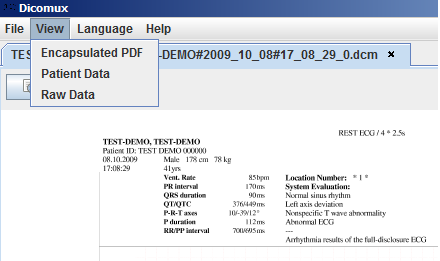
\includegraphics{screens/views.png}}
	\captionof{figure}{Switch views}
	\label{fig:bild}
	\end{minipage}

\section{Open dicom file}
For opening a dicom file click Open Dicom File. You have to choose a dicom file
and click Open. If the chosen file is a correct dicom file DICOMUX loads the
file with its views into the workspace. After that you can switch between the
available views.\\

\begin{minipage}{\textwidth} 
\centering
\fbox{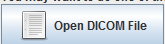
\includegraphics{screens/openFileButton.png}}
\captionof{figure}{Open dicom file}
\label{fig:bild}
\end{minipage}

	\subsection{Encapsulated PDF}
	The Encapsulated PDF view shows the pdf of the dicom file. You have the
	possibility to zoom inside the pdf page. Herefore click the zoom button and draw with the
	mouse the rectangle to zoom in.\\
	To abolish the zoom click again the zoom button. \\
	
	\begin{minipage}{\textwidth} 
	\centering
	\fbox{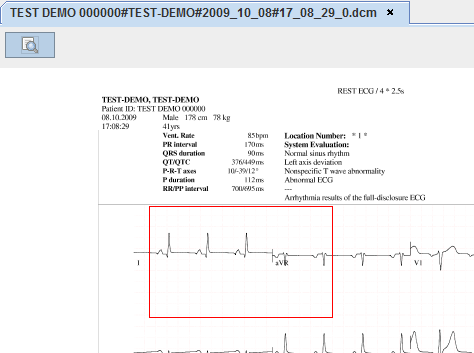
\includegraphics{screens/pdfZoomIn.png}}
	\captionof{figure}{PDF view}
	\label{fig:bild}
	\end{minipage}
	
	\subsection{Waveform ECG}
	The Waveform ECG view shows the ecg data of the dicom file. You can zoom in
	with the plus button, zoom out with the minus button and fit to the page with
	the fit to page button. When you move the mouse over the diplay you can see the
	data of the actual mouse position on the top panel. \\
	There are some different display format options to choose.\\
		
	\begin{minipage}{\textwidth} 
	\centering
	\fbox{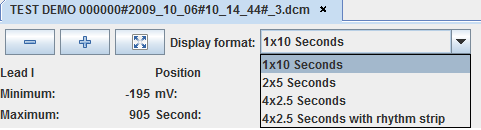
\includegraphics{screens/waveFormFormats.png}}
	\captionof{figure}{Waveform formats}
	\label{fig:bild}
	\end{minipage}
	
		\subsubsection{1x10 Seconds}
		This display format shows 10 seconds of every lead in one row. All leads are
		among each other.
		
		\subsubsection{2x5 Seconds}
		This display format shows 5 seconds of every lead. The leads are displayed in
		two columns. the firts 5 leads are in the first column and the second 5 leads
		are in the second column.\\
		
		\begin{minipage}{\textwidth} 
		\centering
		\fbox{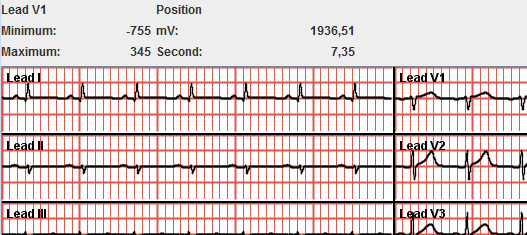
\includegraphics{screens/2x5.png}}
		\captionof{figure}{Display format 2x5}
		\label{fig:bild}
		\end{minipage}
		
		\subsubsection{4x2.5 Seconds}
		This display format shows 2.5 seconds of every lead. The leads are displayed
		in four columns. The firts three leads are in the first column, the second 3
		leads are in the second column, etc..\\
		
		\begin{minipage}{\textwidth} 
		\centering
		\fbox{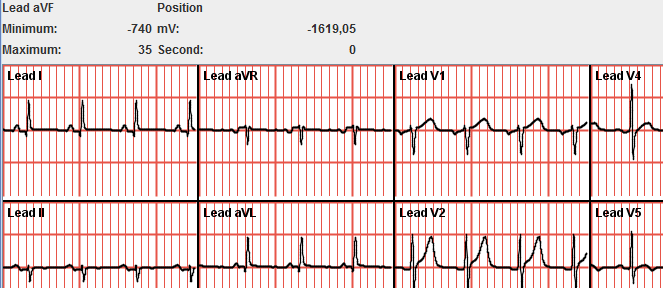
\includegraphics[scale=0.8]{screens/4x25.png}}
		\captionof{figure}{Display format 4x2.5}
		\label{fig:bild}
		\end{minipage}
		
		\subsubsection{4x2.5 Seconds with rhythm strip}
		This display format shows 2.5 seconds of every lead. The leads are displayed
		in four columns. The firts three leads are in the first column, the second 3
		leads are in the second column, etc..\\
		A rhythm strip is shown at the buttom of the display. 10 seconds of the rhythm
		strip are displayed in one row. \\
		
		\begin{minipage}{\textwidth} 
		\centering
		\fbox{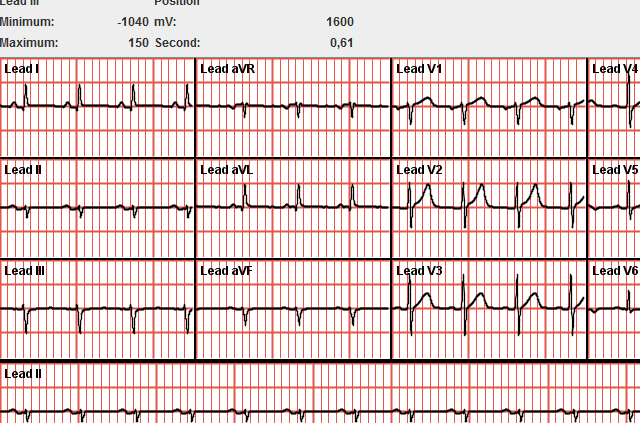
\includegraphics[scale=0.8]{screens/4x25Strip.png}}
		\captionof{figure}{Display format 4x2.5 with rhythm strip}
		\label{fig:bild}
		\end{minipage}

	\subsection{Raw Data}
	The Raw Data view shows all elements of the dicom file with tag address, VR,
	tag name, length and the first couple of the Data characters.
	If an element contains more elements the view shows a folder containing the
	elements.\\
	After you marked an element with data you can view the complete content
	by clicking on the detail button at the top. If the element has no data you
	cannot do that.\\
	
	\begin{minipage}{\textwidth} 
	\centering
	\fbox{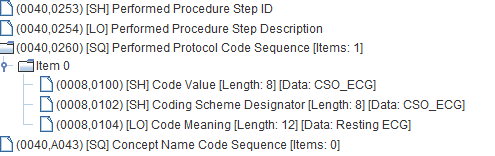
\includegraphics{screens/rawDataStructure.png}}
	\captionof{figure}{Raw data}
	\label{fig:bild}
	\end{minipage}
		
		\subsubsection{Detail view}
		The detail view displays the complete content of the element. You have the
		option to save the content by clicking on the save button. This makes it
		possible to save also an encapsulated pdf in a separate file.
		To return to the Raw Data view click the return button.\\
		
		\begin{minipage}{\textwidth} 
		\centering
		\fbox{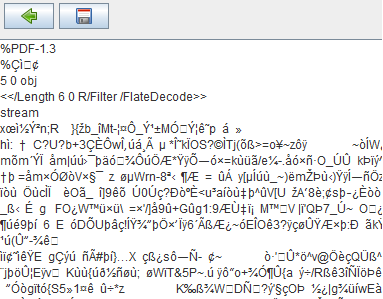
\includegraphics{screens/rawDataDetails.png}}
		\captionof{figure}{Raw data detail view}
		\label{fig:bild}
		\end{minipage}
		
	\subsection{Patient Data}
	The Patient Data view displays information about the patient of the dicom
	file.\\
	
	\begin{minipage}{\textwidth} 
	\centering
	\fbox{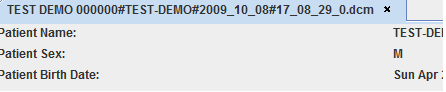
\includegraphics{screens/patientData.png}}
	\captionof{figure}{Patient details}
	\label{fig:bild}
	\end{minipage}
	
\section{Open dicom directory}
To open a dicom directory goto Open Dicom Directory and choose the directory
file. After you chose a correct directory file DICOMUX loads the directory
structure into the workspace.\\
There are four combo boxes showing patient, studies, series and images. By
choosing an entry of a combobox you can navigate to the chosen entry.\\

\begin{minipage}{\textwidth} 
\centering
\fbox{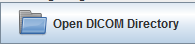
\includegraphics{screens/openDir.png}}
\captionof{figure}{Open dicom directory}
\label{fig:bild}
\end{minipage}

	\subsection{Patient}
	After choosing the entry of patient you can see the information of the
	patient. If you choose a patient the combo boxes series and images are not
	visible anymore. For these you have to choose a study first.
	
	\subsection{Studies}
	After choosing an entry of studies you can see the information of the chosen
	study. The combo box images is not visible. To view the images you have to
	choose a series.\\
	
	\begin{minipage}{\textwidth} 
	\centering
	\fbox{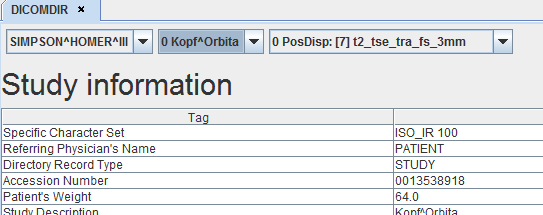
\includegraphics{screens/studyInfo.png}}
	\captionof{figure}{Study information}
	\label{fig:bild}
	\end{minipage}
	
	\subsection{Series}
	After choosing an entry of series you can see the information of the chosen
	series. To view an images you have to choose an entry of the combo box
	images.\\
	
	\begin{minipage}{\textwidth} 
	\centering
	\fbox{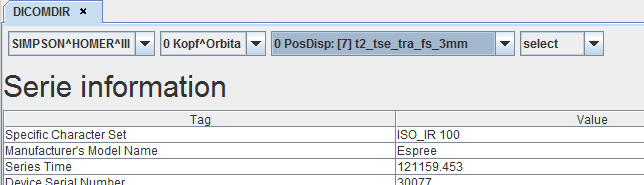
\includegraphics[scale=0.8]{screens/seriesInfo.png}}
	\captionof{figure}{Series information}
	\label{fig:bild}
	\end{minipage}
	
	\subsection{Images}
	After choosing an entry of images the chosen image is shown in the main
	panel.\\
	
	\begin{minipage}{\textwidth} 
	\centering
	\fbox{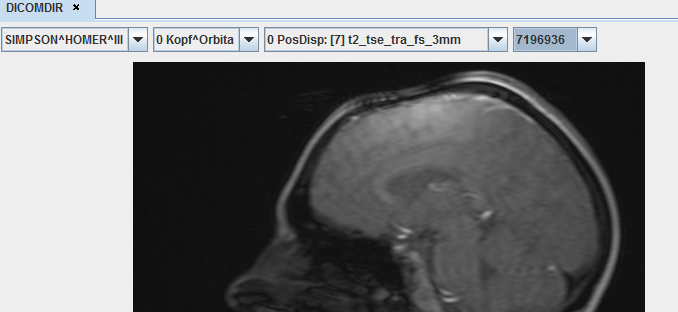
\includegraphics[scale=0.8]{screens/directoryImage.png}}
	\captionof{figure}{Directory Image}
	\label{fig:bild}
	\end{minipage}
	
\section{Language}
DICOMUX provides multilingualism. For changing the language goto the menu entry
Language and choose a language. After you chose a language DICOMUX changes the
language of the menu and the workspaces.\\

\begin{minipage}{\textwidth} 
\centering
\fbox{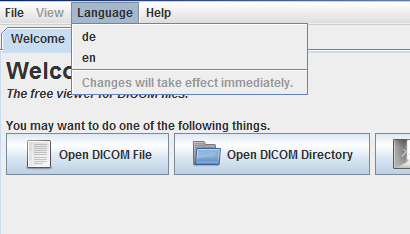
\includegraphics{screens/language.png}}
\captionof{figure}{Change language}
\label{fig:bild}
\end{minipage}

%
% EOF
%